% Percent signs are comments.

% We start with the preamble.  This is the section where you load packages
% (these are like python modules), styles, and define the document.

% Let's define a document.  Other built-in types are book, slide, letter,
% report, etc.
\documentclass[12pt, letterpaper]{article}
% Note the form of a latex command: a backslash, the command name, 
% and two sets of arguments.  In curly braces, we see the actual argument.
% In the brackets, we see options relevant to that argument.  Here, we set
% the document class (article) and two options relevant to that argument
% (font size and paper type).


% Packages expand capabilities in the current document.  To include a package,
% place the package style file (*.sty) into the directory you are working in.
% Better yet, install the package along side your LaTeX installation.  There
% are several ways to do this, I find package managers to be the easiest.
% More info here: https://en.wikibooks.org/wiki/LaTeX/Installing_Extra_Packages
% Let's load some packages:
\usepackage{graphicx} %Allow graphics.
\usepackage{lineno}   %Latex will complain if the lineno.sty file is not in PWD.
\usepackage[authoryear]{natbib}   %More cite commands, author-year format.

% I found that pdflatex, my favorite weapon-of-choice, was goofing my 
% margins.  These commands fix that:
% Force pdflatex to use correct paper size.
%\special{papersize=8.5in,11in}
%\setlength{\pdfpageheight}{\paperheight}
%\setlength{\pdfpagewidth}{\paperwidth}
%%%NOTE- COMMENTED OUT AS NEWER VERSIONS OF TEXLIVE DO NOT HAVE THIS PROBLEM.

% I want my own command to create the backslash character:
% The command's name is ``bslash''; it has zero arguments; when called, it
% simply performs the ``\textbackslash'' function.
\newcommand{\bslash}[0]{\textbackslash}

% I want another command to take two arguments and put them into mathematical
% function notation.  The function name is \func, it has two arguments, and it
% puts the arguments into a math-mode statement.  The #1 and #2 are where 
% arguments one and two are placed.  Examples can be see in the section
% ``make yer own commands''.
\newcommand{\func}[2]{$f(#1)=#2$}

% Eventually, we want to get to work.  We do this by entering the document
% environment like so:
\begin{document}

% Set up title page.
\title{\LaTeX: Greatest Thing Evar}
\author{D. T. Welling\\PHYS 5391} % double-slash for new line.
\date{\today}  % the \today command inserts today's date.

% Create both title page and contents.
% Use page breaks.
\maketitle
\newpage
\tableofcontents
\newpage

% Everything in Latex is some sort of environment.  \begin is a big part
% of what you'll do.

% The lineno package gives us new commands that weren't available before.
% For example, let's turn on our line numbers.
\linenumbers

% Let's start a section.  Sectioning is easy!
\section{Basic Text}
% I can also do subsection, subsubsection, chapter, part, etc.


Here is our first text.  We just type away!
One carriage return will NOT start a new paragraph.  But...

...two will.  I can use \textbackslash noindent to prevent a new paragraph...

\noindent
...started here, from indenting.  There are a LOT of little commands like this.
If I need more space, I can insert a single line by using two slashes.
\\

Tadaa!  Or I can use the vspace command, like so:
\vspace{4mm}

Again, Tadaa!  Note that the vspace doesn't create another line, just space.

Simple special symbols can be created: \& \% \$ \_ and so on.  Escaping
characters is very useful.  If things go wrong, try escaping some characters
that \LaTeX may be confusing for command-like syntax.

Adding emphasis is also easy: \emph{This adds emphasis}, \textbf{this makes
things bold}, \textit{and this makes things italic.}  Note that the 
\textit{emph} command works inside other blocks to add more emphasis:
\textit{we can make italics and then \emph{over emphasize} the text more.}

You can also change the font style mid-sentence:
\texttt{Typewriter script.  Makes for good code examples.}
\textsf{Sans serif.  Makes for... something.}
\textsc{I am so very angry.}

\LaTeX gives you minute control over spacing inside of a paragraph.  For 
example, to get a normal space after a period, use a backslash:

etc. and so on. (No slash.)

etc.\ and so on. (Slash.  Slight, but important.)

Tildes (\~\ ) are similar, but prevent line breaks.  The space between Dr. and
Welling in Dr.~Welling will never break across a line.

Super-scripts are easy:  \textsuperscript{Up here}.
\

\section{Math Environment}
Doing math is easy in \LaTeX.  There are a few ways to do it, however.  The
first is with the full math environment:

\begin{math}  
  % Note that \[ and \] would also work instead of \begin and \end (math only.)
  \nabla \cdot B
\end{math}

We can add an official equation:
\begin{equation}
  \label{eq:1}
  \nabla \cdot B
\end{equation}

Note that the ``official'' equation has a number and accepts a label.  
We'll talk about labels soon.

There are so many equation functions and symbols that it is impossible to list 
them all in an example file like this.  But let's make a mess for fun:

\[
\ddot{Q}\stackrel{\mathrm{def}}{=}\int_{0}^{2\pi} 
\left( \frac{\sqrt[3]{x^2+y^2}}{\bar{A}\times\bar{B}} \right) dx
\]

Inline math text is done easily with dollar signs: $math=great$.

\section{Other cool environments}

\begin{quote}
  The \emph{quote} environment will push a whole block of text over by one tab. 
  This is great for delimiting chunks of text that should stand out for some 
  reason or another.
\end{quote}

\begin{center}
  \emph{center} will center a block of text.
\end{center}

\begin{verbatim}
Verbatim is very helpful when writing blocks of example code:
A lot of stuff is written here. 23@#%#$^WERGSERYE%^*$#^
\end{verbatim}

The tabular environment is super important!
% For tables, you must use a 2nd argument to define the columns.
% the l, c, and r define left, right, or center justification for each
% column.  The vertical bars turn on vertical lines.
\begin{tabular}{l|c|r}
  % For each row, separate the columns with ampersands.
  Col 1 & Col 2 & Col 3\\
  % The \hline command adds a horizontal line.
  \hline
  item 1 & item 2 & item 3\\  % ...don't forget to start a new column
  item 4 & item 5 & item 6\\  % with double-slashes.
\end{tabular}

There are several list environments, too.  For example, 
\begin{itemize}
  \item Bulleted lists
  \item use bullets
  \item to delimit items.    
\end{itemize}

% Note how each item begins with \item.
\begin{enumerate}
  \item To get numbered lists
  \item use the {\tt enumerate} environment
  \item it's great!
\end{enumerate}

Don't forget that you can combine environments to get the result you want.
I like to combine quote and verbatim for making source code examples:
\begin{quote}
\begin{verbatim}
>>> import spacepy.pybats as pb
>>> mhd=pb.Bats2d('example.dat')
>>> mhd.add_contour('x','y','rho',filled=False)
\end{verbatim}
\end{quote}


\section{Floats}

Note that our table created in the last section wound up in-line.  
That's not very nice.  We need to enter the \emph{table} environment to add 
an ``official'' table that can have a caption, a label, etc.  Let's also add 
some complexity to that you can see how tables work more clearly.  Behold!  
Table \ref{tab:ex1}!

% We'll see more of this syntax explained below (e.g., the !h).
\begin{table}[!h]
  \begin{center}
  \begin{tabular}{|l|c|l r|}
    \hline
    Col 1 & Col 2 & Col 3.1 & Col 3.2\\
    \hline
    \hline
    item 1 & item 2 & item 3.1 & item 3.2\\
    item 4 & item 5 & item 6.1 & item 6.2\\
    \hline
  \end{tabular}
  % Caption and label commands are key.
  \caption{An official table that we will use.}
  \label{tab:ex1}
  \end{center}
\end{table}

We did some little things: added a captions, used references and labels (
see Section \ref{sec:cross}), and changed our lines and the number of columns.
The result?  A numbered, caption table placed neatly where it fits.

But how do we know where \LaTeX will put it?  Tables, figures, and other 
objects that should not be broken across a page break (unlike paragraphs) are 
known as \emph{floats}, and \LaTeX has its own rules for where to put them.  
We can give suggestions, as we did in the declaration of our table:
\begin{quote}
\begin{verbatim}
\begin{table}[!h]
\end{verbatim}
\end{quote}
The {\tt !h} option says to put the float ``here'', or as close as you can 
without  making the document look like an idiot put it together.  Adding the 
exclamation point tells \LaTeX to take this suggestion more strongly than 
normal at the cost of making the document layout look crappier.  Other options 
we could have used are {\tt t}, {\tt b}, or {\tt p} for top of page, bottom of 
page, or on a special page at the end of the document.  There are advanced 
float placement rules, including rules for wrapping text around it, etc., 
but we won't tackle that today.


\section{Figures}

Figures can be tricky.  First, you need to turn on the \emph{graphicx} package.
Next, you must know that latex interpreters have limitations.  The standard 
\LaTeX interpreter, {\tt latex}, will accept PDF and PostScript (PS) type 
pictures.  My favorite, {\tt pdflatex}, will take PDF or PNG.  Let's go ahead 
and add a pic; see comments in the source file for details.  Behold!  
Figure \ref{fig:dog}!

\begin{figure}[!b] % I want this picture at the bottom of a page.
\begin{center}
  % This command adds the picture.  The optional arguments can resize, rotate, 
  % flip, and do other operations on the picture.  The required argument is the 
  % figure itself.  You can list a figure in any folder so long as you list the
  % proper path.
  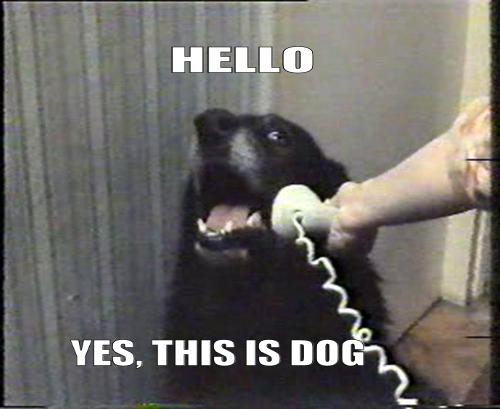
\includegraphics[width=8cm]{dogphone.png} 
  \caption{Get off the phone, dog.}
  \label{fig:dog}
\end{center}
\end{figure}

\section{Cross-reference!}
\label{sec:cross}

Throughout this fake document, I've been able to reference certain sections, 
figures, and tables.  I haven't done this in a hard-coded manner (e.g., in a 
way such that if the order of the sections or figures changes, I would be 
required to change every instance where I refer to that item).  Rather, I've 
been using the \emph{label} environment.  This allows me to use the command 
{\tt \bslash label} to label a figure or section, then use {\tt \bslash ref} to
reference it using the label.  See the source code for examples.

There are some catches, however.  If you don't put your label command in the 
correct spot, especially for floats (figures, tables, etc.), \LaTeX won't use 
the correct number.  The key is to put the label command \emph{after} the 
caption and in the \emph{same environment} as the item you are trying to label.

A final note on references: often, you'll run \LaTeX on your source file only 
to have it complain that it could not find certain labels used in your 
references.  Typically, you just need to run the interpreter one more time and 
you'll be fine.

\section{Source Compilation}
\label{comp}
So far, we have a nice way to make complicated source code with lots of
esoteric rules and slashes.  How do we turn that into a formatted PDF file?
Let's look at what happens at the \emph{terminal} via a set of manual commands.
From the directory that contains your source file, use this command:
\begin{quote}
\begin{verbatim}
latex example.tex
\end{verbatim}
\end{quote}
If everything has gone correctly, you see a whole bunch of new files in your
folder: {\tt example.log}, {\tt example.aux}, and {\tt example.dvi}.  The
last one, the {\tt dvi} file, is a \emph{Device Independent} output file.
This needs to be converted into a PDF or another format via a call to another
program (e.g., {\tt dvipdf}).  That's not very helpful!  Let's use a different
program, {\tt pdflatex}, to produce a PDF right away:
\begin{quote}
\begin{verbatim}
pdflatex example.tex
\end{verbatim}
\end{quote}
Now we see a real PDF file with our output!  Good.  If you have a lot of
cross-references in your file, you may notice that these don't work in
your PDF.  That's fine, just run {\tt pdflatex} again to fix all referencing.
\textbf{When making a final document, always run the compilation step more
  than once to make sure all references and cross references work.}  It takes
\LaTeX \ two passes to do it right: once to make a list of all of the labels
and references (saved in the {\tt .aux} file) and once to include them in the
final PDF.  Always look at the output from the compilation step to make sure
there are no warnings about references!

What's that?  You don't have a PDF?  Something probably went wrong.  That's
okay.  When something goes wrong with \LaTeX , it usually asks for more info
by first posting an error, then printing a question mark and waiting for the
user's response.  Here's an example that we get by purposely introducing a
typo:
\begin{quote}
\begin{verbatim}
! Undefined control sequence.
l.137 \en
         {quote}

?
\end{verbatim}
\end{quote}

When the dreaded ``{\tt ?}'' comes up, you can usually respond with {\tt q} then
pressing enter.  This tells \LaTeX \ to give up for now.  If you continue to
press enter, you will keep getting a list of issues until \LaTeX \ reaches the
end of the file.  It's usually best to just quit and fix the first problem
first.  When you have an issue, keep these things in mind:

\begin{itemize}
\item Start by locating the line number of the problem.  In the above example,
  our line number is {\tt l.137}, or line 137.
\item \emph{READ} the error message.  They can be esoteric, but often \LaTeX \
  is telling you exactly what is wrong.
\item \emph{ALWAYS} fix the first problem first.  Errors cascade such that one
  issue will cause many more.  Fix the first one and many more will disappear.
\item Look for simple but common errors.  Did you mispell a command?  Did you
  forget to close out an environment with an {\tt end} command?  Are you
  missing a special package or style file required in your document?
\item Isolate the issue. If you comment out the line that is causing the
  problem, does it still happen?  Can you narrow it down to a certain spot
  in that line?  Once you know the exact issue, Google it!
\end{itemize}

A final note on compilation: the steps above are for working from the command
line.  Special editors, such as TeXShop, will have buttons to push and
settings to play with to get the output just right.  I recommend feeling out
these programs by creating really simple example files and testing compilation
out on those.

\section{Make yer own commands.}

Making your own commands is easy and right useful.  As an example, above, 
rather than use the verbose {\tt \bslash textbackslash}, I created a shorter 
command called {\tt \bslash bslash} that does the same thing with half of the 
typing.  Making commands with variable arguments is possible, too.  Here's the 
result of a command called {\tt \bslash func}, which inserts arguments into the
correct position in a simple mathematical function: 
\func{2x}{26}; \func{36}{x-y}.  Again, see the source code for details.

\section{Title pages, etc.}
There are built-in tools for making title pages, contents, etc.  See the
commands in the source code; be sure to use {\tt \bslash newpage} to ensure
each winds up on its own page.

\section{Making Bibliographies}
It's possible to do the bibliography by hand, but that's for suckers.  Are
you a sucker? NO!  Use BibTex, fool.  

\subsection{Bibtex Files}
A bibtex file contains all of the info for 
any references you may use in the following format:

\begin{quote}
\begin{verbatim}
@ARTICLE{welling:2010c,
   author = {{Welling}, D.~T.},
    title = "{The long-term effects of space weather on satellite operations}",
  journal = {Annales Geophysicae},
     year = 2010,
    month = jun,
   volume = 28,
    pages = {1361-1367},
      doi = {10.5194/angeo-28-1361-2010}
}
\end{verbatim}
\end{quote}

This is an {\it article} entry, but you can also make {\it book}, 
{\it conference}, {\it inproceedings}, and other entries.  There are many other
fields that can be filled in to make your entry more complete.  

\subsection{Building Bibtex Files}
There are many sources for getting bibtex entries.  Typically, your research 
group or advisor will have a standard one that contains most everything.  
Many websites that list articles will have corresponding bibtex entries to save
you the hassle of building them manually.  Other times, you'll just have to add
an entry by yourself.  In the end, you'll have a running bibtex file that grows
as you write more.

\subsection{Citations}
The label {\tt welling:2010c} is how you reference a citation in \LaTeX.  For 
example, to reference \cite[p. 13]{welling:2010c} in the text, I typed 
\verb+\cite[p. 13]{welling:2010c}+ voila!  Citation acheived.  This sentence is
very important \cite[]{dungey1961,axford1961,Parker:1960}.
There are other commands,
such as {\tt \bslash citet}, which puts the citation in the sentence and does 
not bracket it off.  There is also {\tt \bslash citep}, which creates a
parenthetical citation.
{\tt \bslash nocite} will ensure the cited work winds up 
in the bibliography without creating an inline-citation.
Example: \citet{welling:2011} said that dogs sometimes eat potatoes.
He was wrong.  The {\tt \bslash citep} and {\tt \bslash citet} commands often
work much better than the plain {\tt \bslash cite} command, so I recommend
using those.  However, there is one extra step required to use these:
To get these extra  commands, we must use an additional
package, {\tt natlib}.  As such, the following command appears in this
document's preamble:

\begin{quote}
\begin{verbatim}
\usepackage[authoryear]{natbib}
\end{verbatim}
\end{quote}

\noindent ...where the {\tt authoryear} syntax specifies that I want to cite
by author-year.  Other options inlcude {\tt apalike}, {\tt alpha}, and others.
Look them up!

\subsection{Building the Bib}
Once you have a bibtex file and have created all of the citations, put this at 
the end of your article (or where you wish to put your bibliography):

\begin{quote}
\begin{verbatim}
\bibliographystyle{plainnat}
\bibliography{sample_bib}
\end{verbatim}
\end{quote} 

These commands point to the bibliography style files (\emph{must} end in 
{\tt .bst}) and your bibtex file (\emph{must} end in {\tt .bib}).  There are 
some built in bibliography files, but typically you are given a particular file
 from a journal.  Here, we're using the built-in bibstyle, {\tt plainnat.bst}.
This is included with the natlib package.  If it wasn't, we would need that 
file either installed in the correct \LaTeX folder or placed in the current
working directory.

Compilation becomes a bit more difficult.  First, run your \LaTeX interpreter 
once.  There will be much gnashing of teeth as \LaTeX won't know what to do 
with your citations.  That's fine; ignore it.  Next, run bibtex as follows:

\begin{quote}
\begin{verbatim}
bibtex example
\end{verbatim}
\end{quote}

\emph{Note that we did NOT use the file extension!}  Finally, run your \LaTeX\ 
interpreter again; two more times if you want to be thorough.   Here, it's good
to start using a Makefile to make your life easier.  You'll notice that bibtex 
creates a bunch of new files, notably {\tt example.bbl}.  
\emph{This file is your bibliography}, and if you open it, you'll see what you 
must type into your file manually if you don't use bibtex!

Finally, run your \LaTeX interpreter once (or twice for cross-references) more 
to finish your document.  Beautiful!  Note that using the plain bib-style and 
the Article document class, References did not get its own section.  It's 
possible to force this, either by changing document class, using a different 
bib style, or using a combination of commands to force \LaTeX to do your 
bidding (you'll note that we have taken that route in the source file.)

\section{Other Crap}
You can do damn near anything in \LaTeX, just be sure to GDS (the golden rule of
programming).  Two columns, text wrapping around figures and tables, different
fonts, advanced tabbing, etc. are all possible.  It's possible to create your
own stuff, but this is usually not necessary- someone has likely done it before.

% These two lines force a new page and a section in the table of contents
% for the bibliography.  Very useful.
\clearpage
\addcontentsline{toc}{section}{Bibliography}
% Using Bibtex, we just use these two lines to add the bib!
\bibliographystyle{plainnat}
\bibliography{sample_bib}

% End the document environment.  No other lines will be read after this point.
\end{document}
